\section{Description}
\subsection{Motivation}
As an example, many arrests and court cases hinge on the finding of recovered files like the infamous Craigslist 
Killer. Data from deleted files can prove ones’ innocence or guilt just as much as DNA proof can. Information 
like created times, who wrote the file, and even past versions can make or break a case for law enforcement. 
Having knowledge of which software will perform best for each instance can save a lot of time for investigators to find the guilty party.

\subsection{Preliminary Findings}
I have already done a set of experiments with Autopsy tool against the CFTT Core standards with one filesystem. 
This experiment showed it is possible to replicate the same process multiple time for each software to test. 
This experiment also showed the value of changing the complexity of how the files were deleted. 
Sometimes a new file can overwrite the desired deleted file, and it has to be pieced back together. 

\subsection{Testing Plans}
My desktop is powerful enough (i7 8700k CPU, 32GB RAM, GTX 1060 GPU) to run multiple instances of virtual machines 
that I can test with multiple Operating Systems(Windows, Mac and Linux). Using these virtual machines, I can also test multiple file types 
(Pictures, Word Docs, PDFs, etc.). See Figure\ref{fig1} below for diagram of testing setup.

%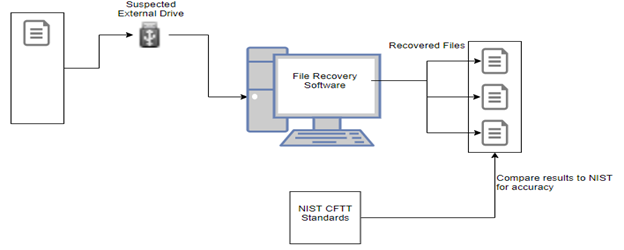
\includegraphics[scale=0.4]{./figs/fig1.png}

\begin{figure}[t] \label{fig1}
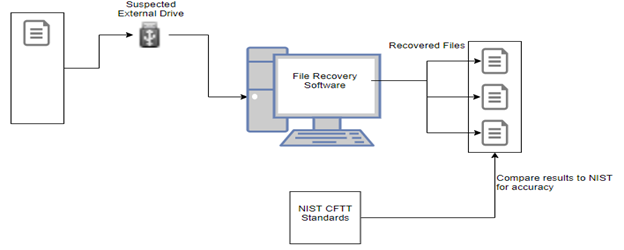
\includegraphics[width=10cm]{./figs/fig1.png}
\centering
\end{figure}

I plan to test with popular free and paid versions of popular open source and enterprise file recovery software to 
show if the open source maintains the same standards This can also help future students in understanding the difference in 
capabilities that different software has. Some example software that I plan to use are 
Recuva, PhotoRec, Magnet Axiom, FTK or EnCase, \sr{We should select two free (autopsy and something) and two enterprise (magnet and ftk).} 
\qc{Removed some tools and left open for more if I have the time}
and others as possible. By testing multiple tools on multiple operating systems, it will give a universal resource for 
others to understand the various software capabilities and restrictions. 

\subsection{Reporting}
The CFTT already has a few published reports of different file recovery software. However, they should be expanded and 
retested to ensure their reliability is consistent as new patches and features come out for file recovery tools. By 
adding new reports to the website that other researchers can test and confirm will allow developers a chance to continually 
develop their tool for the better.

\section{Anticipated Outcomes}
I anticipate the free consumer tools will not meet as many standards compared to the professional or more complex software 
because the time and effort developing them. Each software I will be testing is unique in their own way, 
but when providing a use to recover a deleted file, the CFTT Standards act as a guideline to what 
the software should retrieve. I estimate that while there are more tools for windows file systems, the ones 
developed primarily for Linux will have the most versatility and highest passing mark for recovering files.\sr{We also aim to find out possible underlying causes of failure of a tool in a scenario, which can lead to better design of future tools.} 

I aim to turn this research into a published paper with the assistance of Professor Roy if I am able 
to discover enough information about the various tools. I am hoping that this will inspire future readers to test 
different software for themselves and show the importance of having a standard that can be used to \emph{grade} a software.
As students look more and more into file recovery, relating software back to which standards they pass will help students 
understand why the standards are important and what can happen to deleted files if they do not pass. 

